\chapter{数值方法} \label{chap4}
\section{引言}
在前文给出连续的控制方程,以及表面重建方法后,本章将离散化连续控制方程,以及针对
流体表面张力给出一个物质的离散化方式,同时给出一个计算流水线将表面重建方法整合到物质点法中来完成我们的模拟。
\section{离散控制方程}
我们将使用伽辽金方法离散化控制方程,首先我们先将第一章中的动量强形式方程转换成弱形式,然后根据弱形式选取基函数以及
对应的离散方法用于数值计算。此处我们回顾动量守恒方程的欧拉形式和拉格朗日形式,
\begin{align*}    
    &\rho \frac{Dv}{Dt} = div(\sigma) + \rho g & \text{欧拉视角}\\
    &R(X,0)\frac{\partial}{\partial t} V(X,t) = DIV(P) + Rg &\text{拉格朗日视角}
\end{align*}
其中$v(x,t) = V(X,t), x = \phi(X,t)$。如果我们从拉格朗日视角来观察方程的左侧(时间变化项),从欧拉视角来观察方程的右侧(空间变化项),
那么我们有如下混合欧拉拉格朗日形式的方程
\begin{align*}
    &R(X,0)\frac{\partial}{\partial t} V(X,t) = div(\sigma) + \rho g & \text{混合欧拉拉格朗日视角}\\ 
\end{align*}
\subsection{时间离散化}
在混合欧拉拉格朗日视角中,左端项为$R(X,0)\frac{\partial}{\partial t}V(X,t)$,相对于欧拉视角下$\rho \frac{Dv}{Dt}$中的材料时间导数
$\frac{D}{Dt} = \frac{\partial}{\partial t} + v\cdot \nabla$,显然有更容易的离散方式,这也是时间变化项选择拉格朗日描述的原因。
此处我们使用有限差分来离散速度有关时间的变化。
\begin{align*}
    \frac{\partial}{\partial t} V(X,t) \approx \frac{V(X,t^{n+1}) - V(X,t^n)}{\Delta t}
\end{align*}

同样的,在拉格朗日视角下的离散化可以转换为欧拉视角下的离散化,这里记$x^{n} := \phi_{t^n}(X)$, $\hat{x}^{n+1} := \phi_{t^{n+1},t^n}(x^n)$,同时
$v^n(x^n) := v(x^n,t^n), \hat{v}^{n+1}(x^n) := v(\phi_{t^{n+1},t^n}(x^n))$,因此以上差分格式可以写成
\begin{align*}
    \frac{\partial}{\partial t} V(X,t) \approx \frac{\hat{v}^{n+1}(x^n) - v^n(x^n)}{\Delta t}
\end{align*}
值得注意的是,$\hat{v}^{n+1}(x^n)$与$v^n(x^n)$都是在$\Omega^{t^n} = \phi_{t^n}(\Omega^0)$上定义的,因此该离散形式既可在欧拉视角下表示,同时也可以在
拉格朗日视角下表示。
\subsection{弱形式}
将左端形式带入欧拉视角中,我们有如下
\begin{align*}
    \rho(x^n,t^n)\frac{\hat{v}^{n+1}(x^n) - v^n(x^n)}{\Delta t} = div(\sigma) + \rho g
\end{align*}
为了将表面张力融入方程中,我们补充边界条件如下
\begin{align*}
    \rho(x^n,t^n)\frac{\hat{v}^{n+1}(x^n) - v^n(x^n)}{\Delta t} &= div(\sigma) + \rho g \\
    \sigma n &= t, x^n \in \partial \Omega^{t^n}\\
\end{align*}
上述方程以弱形式表示我们有,这里$w$选取为空间上具有紧支集的测试函数
\begin{align*}
    \int_{\Omega^{t^n}}\rho(x,t^n)\frac{\hat{v}^{n+1}(x) - v^n(x)}{\Delta t}\cdot wdx &= \int_{\Omega^{t^n}} div(\sigma)\cdot w dx + \int_{\Omega^{t^n}}\rho g\cdot w dx\\
    \sigma n &= t, x \in \partial \Omega^{t^n}\\   
\end{align*}
现在我们处理右端的散度项,由格林公式[**]得
\begin{align*}
    \int_{\Omega^{t^n}} div(\sigma)\cdot w dx &= \int_{\partial \Omega^{t^n}}w\cdot (\sigma n) ds - \int_{\Omega^{t^n}} \sigma : \nabla w dx\\
        &= \int_{\partial \Omega^{t^n}}w\cdot t ds - \int_{\Omega^{t^n}} \sigma :\nabla w dx
\end{align*}
我们先计算$\int_{\partial \Omega^{t^n}}\sigma : \nabla w dx$部分。回顾流体弱可压缩模型获得的柯西应力$$\sigma = \lambda (det(F) - 1)I$$带入可得
$\int_{\partial \Omega^{t^n}} \lambda (det(F) - 1) I:\nabla w dx$。
将上式整合我们得到
\begin{align*}
    \int_{\Omega^{t^n}}\rho(x,t^n)\frac{\hat{v}^{n+1}(x) - v^n(x)}{\Delta t}\cdot wdx &= \int_{\partial \Omega^{t^n}} w\cdot t ds - \int_{\Omega^{t^n}} \sigma:\nabla w dx
\end{align*}
为了计算表面张力项,回顾我们在第一章得到的表面张力计算公式
$$S(\phi_{t}) = k \int_{\partial \Omega_{t^n}} det(F(x;t,t^{n})) \Vert F^{-T}(x;t,t^{n})\tilde{n}\Vert d\tilde{s}$$
我们对其变分将获得流体表面上的表面张力场。为了方便,我们先记$\tilde{F} = F(x;t,t^n)$,以及$\Psi(\tilde{F}) = det(\tilde{F})\Vert \tilde{F}^{-T}\tilde{n} \Vert$,则
\begin{align}
    \delta \Psi(\tilde{F}) &= \delta(det(\tilde{F})\Vert \tilde{F}^{-T}\tilde{n} \Vert) \nonumber\\
    &= \delta[det(\tilde{F})] \Vert \tilde{F}^{-T} \tilde{n} \Vert + det(\tilde{F})\delta \Vert \tilde{F}^{-T}\tilde{n} \Vert \nonumber\\
    &= det(\tilde{F})\tilde{F}^{-T}:\delta \tilde{F} \cdot \Vert \tilde{F}^{-T}\tilde{n}\Vert + det(\tilde{F})\delta \Vert \tilde{F}^{-T} \tilde{n} \Vert
\end{align}
这里第三行我们使用了第二章提到的行列式求导结果$\delta det(F) = det(F)F^{-T}:\delta F$,接下来我们处理上述等式的右端项
$\delta \Vert \tilde{F}^{-T}\tilde{n}\Vert$。这里注意到$\Vert V \Vert^2 = V^TV$,因此我们有$2\Vert V\Vert \delta \Vert V \Vert = 2V^T\delta V$。
同时$A^{-1}A = I$,从这里我们由$\delta A^{-1} A + A^{-1}\delta A = 0$,整理得到$\delta (A^{-1}) = - A^{-1}\delta A A^{-1}$。那么我们由
\begin{align*}
    \delta \Vert \tilde{F}^{-T}\tilde{n}\Vert &= \frac{\tilde{n}^{T}\delta(\tilde{F}^{-1})\tilde{F}^{-T}\tilde{n}}{\Vert \tilde{F}^{-T}\tilde{n}\Vert}\\
    &= \frac{-\tilde{n}\tilde{F}^{-1}(\delta \tilde{F})\tilde{F}^{-1}\tilde{F}^{-T}\tilde{n}}{\Vert \tilde{F}^{-T}\tilde{n} \Vert}
\end{align*}
将上式带入(4.1)式得
\begin{align*}
    \delta \Psi(\tilde{F}) = det(\tilde{F})\tilde{F}^{-T}:\delta \tilde{F} \cdot \Vert \tilde{F}^{-T}\tilde{n}\Vert - \frac{\tilde{n}^T\tilde{F}^{-1}(\delta \tilde{F})\tilde{F}^{-1}\tilde{F}^{-T}\tilde{n}}{\Vert \tilde{F}^{-T}\tilde{n} \Vert}
\end{align*}
则
\begin{align*}
    \delta \Psi (F(x_0;t_0,t_0)) &= \delta \Psi(I)\\ 
    &= I:\delta \tilde{F} - \tilde{n}^T\delta \tilde{F} \tilde{n}\\
    &= I:\delta \tilde{F} - \tilde{n}\tilde{n}^T:\delta \tilde{F}\\
    &= (I - \tilde{n}\tilde{n}^T):\delta \tilde{F}
\end{align*}
而表面能量变化等于表面张力沿位移做的功,这里$\delta \phi_{t^n} (X) = w\circ\phi_{t^n}(X)$,即
$$\delta S(\phi_{t^n}) = \int_{\partial \Omega^{t^n}} w\cdot t ds$$
因此我们有
\begin{align*}
    \int_{\partial \Omega^{t^n}} w\cdot t ds &= \delta S(\phi_{t^n})\\
    &= k\int_{\partial \Omega^{t^n}} (I - \tilde{n}\tilde{n}^{T}):\delta \tilde{F}ds\\
    &= k\int_{\partial \Omega^{t^n}} (I - \tilde{n}\tilde{n}^{T}):\nabla w ds\\
\end{align*}

因此我们可以得到
\begin{align}
    \int_{\Omega^{t^n}}\rho(x,t^n)\frac{\hat{v}^{n+1}(x) - v^n(x)}{\Delta t}\cdot wdx = &k\int_{\partial \Omega^{t^n}} (I - \tilde{n}\tilde{n}^T):\nabla w ds\nonumber\\
    & -\int_{\Omega^{t^n}}\lambda (det(F\circ \phi_t^{-1}) - 1)I:\nabla w dx
\end{align}
\subsection{空间离散化}
在得到(4.2)式后我们将积分离散化,首先我们假设$\Omega^{t^n}$被离散为点云$\mathcal{V}$,如图\ref{fig: discretise continuum}所示。
\begin{figure}[htbp]
    \centering
    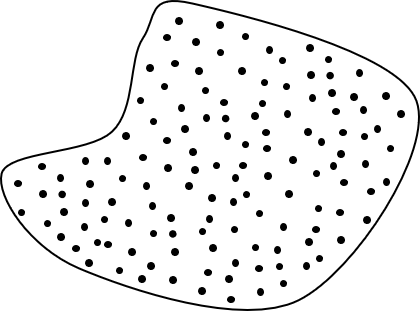
\includegraphics[scale=0.8]{./images/image11.png}
    \caption{连续体离散化成点云}
    \label{fig: discretise continuum}
\end{figure}

其次假设有限元函数空间为$$\{f: f(x) = \sum_\mathbf{i} f_\mathbf{i} B_\mathbf{i}(x), \mathbf{i} = ijk, i,j,k\in{1,2,3}\}$$因此
$\hat{v}^{n+1}(x) = \sum_{\mathbf{i}}\hat{v}^{n+1}_{\mathbf{i}}B_{\mathbf{i}}(x)$,$v^n(x) = \sum_{\mathbf{i}}v^n_{\textbf{i}}B_{\textbf{i}}(x)$,测试函数$w(x) = e_{\alpha}B_{\mathbf{i}}(x)$,这里$e_{\alpha}$为三维空间的第$\alpha\in\{1,2,3\}$个标准基。
带入(4.2)式左边有
\begin{align}
    \int_{\Omega^{t^n}}\rho(x,t^n)\frac{\hat{v}^{n+1}(x) - v^n(x)}{\Delta t}\cdot w dx &=  \int_{\Omega^{t^n}} \rho(x,t^n)\sum_{\mathbf{i}}\frac{\hat{v}^{n+1}_\mathbf{i} - v^n_{\mathbf{i}}}{\Delta t}B_\mathbf{i}(x)\cdot e_{\alpha}B_{\mathbf{j}}(x)dx\nonumber
\end{align}
右边为
\begin{align}
    \int_{\partial \Omega^{t^n}} (I - \tilde{n}\tilde{n}^T):e_{\alpha}\nabla B_{\mathbf{j}}(x) ds - \int_{\Omega^{t^n}}\lambda (det(F\circ \phi_t^{-1}) - 1)I:e_{\alpha}\nabla B_\mathbf{j}(x) dx
\end{align}
如果我们同时考虑$e_{\alpha},\alpha = 1,2,3$,这样上式即在三个维度统一表示为
\begin{align}
    \int_{\Omega^{t^n}}\rho(x,t^n)\sum_\mathbf{i} \frac{\hat{v}^{n+1}_\mathbf{i} - v^n_{\mathbf{i}}}{\Delta t}B_\mathbf{i}(x)B_\mathbf{j}(x)dx &= \int_{\partial \Omega^{t^n}} (I - \tilde{n}\tilde{n}^T)\nabla B_{\mathbf{i}}(x)^T ds \nonumber\\
                                                                            & - \int_{\Omega^{t^n}} \lambda (det(F\circ \phi_t^{-1}) - 1)\nabla B_\mathbf{i}(x)^T dx \nonumber     
\end{align}
对积分离散化我们有
\begin{align}
    \sum_\mathbf{i}\int_{\Omega^{t^n}}\rho(x,t^n) \frac{\hat{v}^{n+1}_\mathbf{i} - v^n_{\mathbf{i}}}{\Delta t}B_\mathbf{i}(x)B_\mathbf{j}(x)dx &\approx \sum_{\mathbf{i},p}B_\mathbf{i}(x_p^n)B_\mathbf{j}(x_p^n)\frac{\hat{v}^{n+1}_\mathbf{i} - v^n_{\mathbf{i}}}{\Delta t}\int_{\Omega^{t^n}_p}\rho(x,t)dx\nonumber\\
    &= \sum_{\mathbf{i},p}B_\mathbf{i}(x_p^n)B_\mathbf{j}(x_p^n)\frac{\hat{v}^{n+1}_\mathbf{i} - v^n_{\mathbf{i}}}{\Delta t}m_p
\end{align}
此处$p\in \mathcal{V}$为离散点云上的点,$x_p^n\in \mathbb{R}^3$为$t^n$时刻点$p$的位置,$m_p = \int_{\Omega_p^{t^n}} \rho(x,t)dx$,这里$m_p$为粒子$p$周围的质量,根据质量守恒,$m_p$与时间无关。
再记$\hat{M}_{\mathbf{j}\mathbf{i}} = \sum_p B_{\mathbf{j}}(x_p^n)B_{\mathbf{i}}(x_p^n)m_p$
通常我们会牺牲精度,使用矩阵行求和的方式[**]来简化矩阵$\hat{M}$。即$M_{\mathbf{jj}} = \sum_{\mathbf{i}}\hat{M}_{\mathbf{ji}}$,$M$的非对角项为0。同时注意到,
B-样条的单位分解性,我们有
$$M_{\mathbf{jj}} = \sum_p m_p B_{\mathbf{j}}(x_p^n)\sum_\mathbf{i}B_\mathbf{i}(x_p^n) = \sum_p m_p B_{\mathbf{j}}(x_p^n)$$
同理我们可以得到
\begin{align}
    \int_{\Omega^{t^n}}\lambda (det(F\circ \phi_t^{-1}) - 1)\nabla B_{\mathbf{j}}(x)^Tdx &\approx \sum_p \lambda (det(F_p^n) - 1)\nabla B_{\mathbf{j}}(x_p^n)^T\int_{\Omega^{t^n}_p}dx \nonumber\\
    & = \sum_p \lambda (det(F_p^n) - 1)\nabla B_{\mathbf{j}}(x_p^n)^T V_p^n\nonumber \\
    & \approx \sum_p \lambda (det(F_p^n) - 1)\nabla B_{\mathbf{j}}(x_p^n)^T V_p^0\nonumber     
\end{align}
这里$F_p^n$为粒子$p$在$t^n$时刻的形变梯度,$V_p^n$为时刻$t^n$时$p$邻域小块$\Omega_p^{t^n}$的体积,由于我们将使用较大的体积惩罚来减小体积变化,因此我们可以近似$V_p^n$为初始时刻的体积$V_p^0$。

最后我们来处理表面积分项$\int_{\partial \Omega^{t^n}} (I - \tilde{n}\tilde{n}^T)\nabla B_{\mathbf{i}}(x)^T ds$,假定我们已经获取了点云在$t^n$时刻的表面,总表面积为$Area$,且已在表面上均匀的采点,每个点分配面积为$A_s = \frac{Area}{\#\mathcal{S}}$,表面点集为$\mathcal{S}$。
\begin{figure}[htbp]
    \centering
    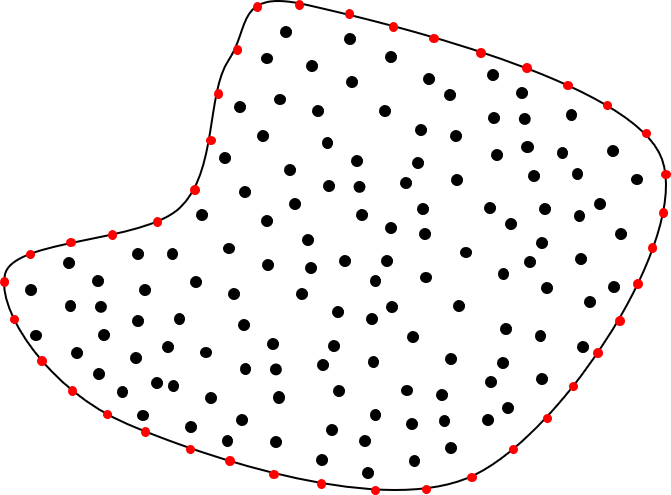
\includegraphics[scale=0.4]{./images/image12.png}
    \caption{红色点$s$为采样获得的表面点集$\mathcal{S}$}
    \label{fig: surface of point cloud}
\end{figure}

那么我们有
\begin{align}
    \int_{\partial \Omega^{t^n}} (I - \tilde{n}\tilde{n}^T)\nabla B_{\mathbf{j}}(x)^T ds &\approx \sum_{s\in\mathcal{S}}(I - \tilde{n}_s\tilde{n}_s^T)\nabla B_{\mathbf{j}}(x_s^n)^TA_s
\end{align}
将上述离散化结果整理我们得到
\begin{align}
    \sum_{p\in \mathcal{V}} \frac{\hat{v}^{n+1}_\mathbf{j} - v^n_{\mathbf{j}}}{\Delta t}m_pB_{\mathbf{j}}(x_p^n) = &k\sum_{s\in\mathcal{S}}(I - \tilde{n}_s\tilde{n}_s^T)\nabla B_{\mathbf{j}}(x_s^n)^TA_s\nonumber\\
    & - \lambda \sum_{p\in\mathcal{V}} (det(F_p^n) - 1)\nabla B_{\mathbf{j}}(x_p^n)^T V_p^0
\end{align}
如果记$m_{\mathbf{j}}^n = \sum_p m_p B_{\mathbf{j}}(x_p^n)$,则上述问题变为
\begin{align}
    m_\mathbf{j}^n \frac{\hat{v}^{n+1}_\mathbf{j} - v^n_{\mathbf{j}}}{\Delta t} &= k\sum_{s\in \mathcal{S}}(I - \tilde{n}_s\tilde{n}_s^T)\nabla B_\mathbf{j}(x_s^n)^TA_s\nonumber\\
    & - \lambda \sum_{p\in\mathcal{V}} (det(F_p^n) - 1)\nabla B_{\mathbf{j}}(x_p^n)^T 
\end{align}
自然我们给出$p$的位置$x_p^n$更新公式
\begin{align}    
    x_p^{n+1} = x_p^n + \Delta t \tilde{v}_p^{n+1}
\end{align}
同时回顾第二章的$\dot{F} = \nabla v \cdot F$,我们得到
\begin{align}
    F^{n+1}_p = (I + \Delta t\cdot \nabla {v}^{n+1}_p)F^n_p
\end{align}

\subsection{数据表示与储存}
从式(4.7),(4.8),(4.9)可以看到,我们需要的变量有$x_p^n\in \mathbb{R}^3,v_p^{n}\in \mathbb{R}^3,F_p^n\in \mathbb{R}^{3\times 3}$,这些变量我们都储存在粒子上,由于粒子上储存质量信息不会随着时间改变,因此该数据表示方式
自然的满足了质量守恒方程。如图\ref{fig: particle information}所示
\begin{figure}[htbp]
    \centering
    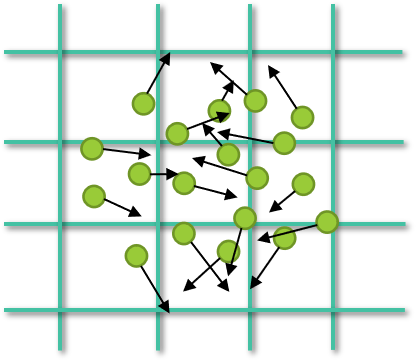
\includegraphics[scale=0.7]{./images/image13.png}
    \caption{粒子上的信息}
    \label{fig: particle information}
\end{figure}

同时注意到这里在$t^n$时刻需要参与计算的信息还有$v_\mathbf{j}^n \in \mathbb{R}^3$和$m_\mathbf{j}^n \in \mathbb{R}$,这里的信息我们储存在
格点上。如图\ref{fig: grid information}所示,这里我们注意到$m_{\mathbf{j}}^n = \sum_p m_p B_{\mathbf{j}}(x_p^n)$,此处实际上我们把粒子上的
数据分散到了网格上,同时注意到$\sum_{\mathbf{j}} m_\mathbf{j}^n = \sum_{\mathbf{j}}\sum_p m_p B_{\mathbf{j}}(x_p^n)$,这里再使用B-样条的单位分解性,我们有
$\sum_{\mathbf{j}}m_\mathbf{j} = \sum_p m_p$,因此该分配方式依然是质量守恒的过程。
\begin{figure}[htbp]
    \centering
    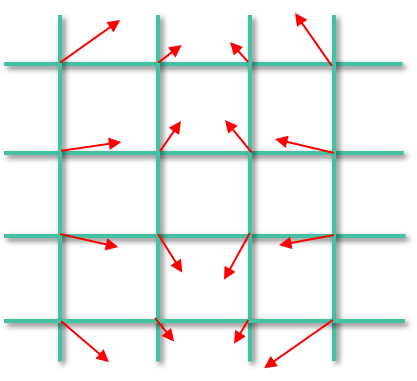
\includegraphics[scale=0.7]{./images/image14.png}
    \caption{格点上的信息}
    \label{fig: grid information}
\end{figure}

\section{数值修正}
在上一节得到连续方程的离散化之后,我们接下来给出该离散方程的计算策略以及一些工程实践上的修正。
\subsection{表面重建与粒子属性调整}
在给定的粒子集合$\mathcal{V}$以及$t^n$时刻每个粒子$p \in \mathcal{V}$的位置$x_p$时,我们可以使用第\ref{chap3}章
提到的方法重建表面网格,然后使用泊松圆盘采样获取表面的粒子$\mathcal{S}$。在构造隐式曲面时,我们需要额外的偏移量,此
处我们对每一个$s\in \mathcal{S}$,在$\mathcal{V}$中寻找距离$s$最近的粒子$p_s \in \mathcal{V}$,偏移方向
为$n_s = \frac{x_s - x_{p_s}}{\Vert x_s - x_{p_s} \Vert}$,如图\ref{fig: offset of surface particle}所示。我们将
$\mathcal{S}$和$\mathcal{N}$作为输入可以得到逼近的隐式曲面,然后估计$S$中表面粒子的法向$\tilde{n}_s$。
\begin{figure}[htbp]
    \centering
    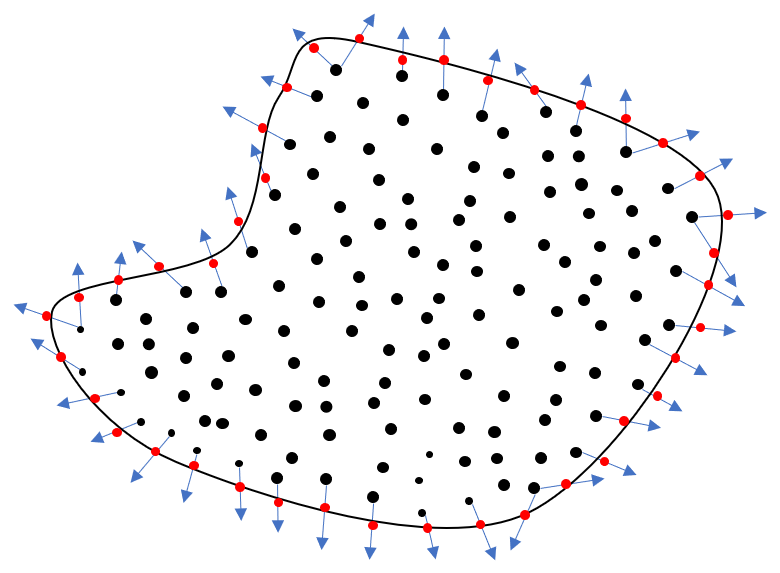
\includegraphics[scale=0.7]{./images/image15.png}
    \caption{箭头为偏移方向,红色点为表面粒子$s\in \mathcal{S}$,箭头起始端为$p_s \in\mathcal{V}$}
    \label{fig: offset of surface particle}
\end{figure}

在实践中,表面张力项$f^{surface} = k\sum_{s\in \mathcal{S}}(I - \tilde{n}_s\tilde{n}_s^T)\nabla B_{\mathbf{j}}(x_s^n)^TA_s$需要传导到内部粒子,与液体压力共同影响形变结果,如果表面粒子离内部粒子最短距离大于
$\sqrt{3}h$(即在$s$所占的一个格子之外),那么该表面粒子$s\in \mathcal{S}$将难以通过网格把表面张力传导到内部粒子。为了解决这一问题,我们对每一个表面粒子$s\in \mathcal{S}$寻找其在内部的最近的点$p_s \in \mathcal{V}$,
然后生成一个嵌入点$o_s$,嵌入点$o_s$的位置我们选取为$x_{o_s} = 2x_{p_s} - x_s$,嵌入点集合我们记为$\mathcal{O}$。显然,$\mathcal{O}$与$\mathcal{S}$有一一对应关系,而内部点$p\in\mathcal{V}$与表面点集可能是多对一,因此我们记录每一个内部点
$v$所相关的表面点个数$C_v$,同时我们将内部点的质量均匀的分布给表面粒子和嵌入粒子,即$m_s = m_{o_s} = \frac{m_{p_s}}{2C_{p_s} + 1}$,其中内部粒子$p_s$的质量$m_{p_s}$重新赋值为$m_s$。同样的,我们赋予当前时刻表面粒子速度$v_s^n = v_{p_s}^n$以及嵌入粒子$o_s$
的速度$v_{o_s}^n = v_{p_s}^n$。
\begin{figure}[htbp]
    \centering
    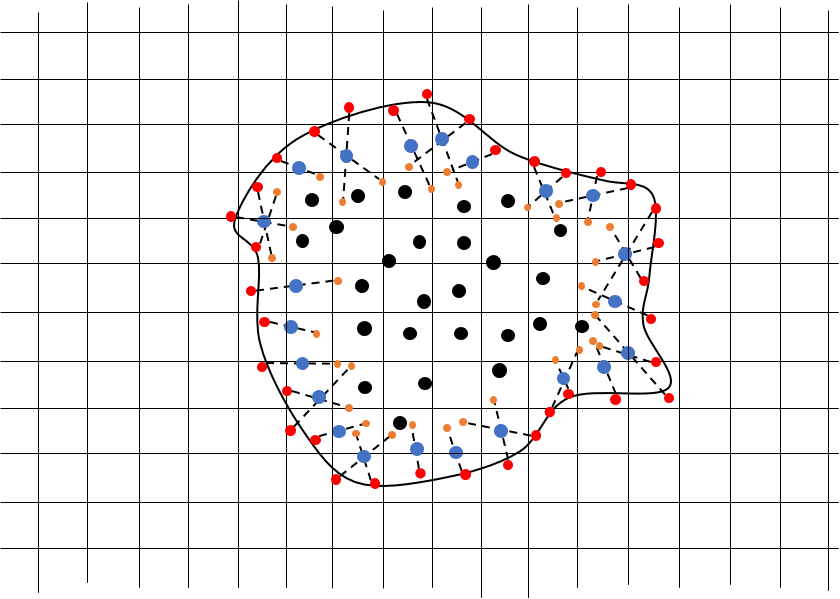
\includegraphics[scale=0.7]{./images/image16.png}
    \caption{红色点为表面粒子$s\in \mathcal{S}$,红色点通过虚线所连的蓝色点为离$s$最近的内部点$p_s\in \mathcal{V}$,橙色点$o_s\in \mathcal{O}$为新嵌入内部点}
    \label{fig: surface particle inserted}
\end{figure}
\subsection{粒子网格信息转换}
实际上在上一节中,我们已经给出了把粒子上的质量信息传递到网格上的计算公式,即$\tilde{m}^n_{\mathbf{j}} = \sum_p \tilde{m}_p B_{\mathbf{j}}(x_p^n)$。除了质量信息之外,我们仍然需要
速度信息$v_\mathbf{j}^n$,基于动量守恒的考虑[**],我们采用的传递方式为将粒子的动量信息传递到网格上,再通过动量和质量的关系获取网格上的速度,即
\begin{align}
    (mv)_\mathbf{j}^n &= \sum_{p} \tilde{m}_p v_p^nB_{\mathbf{j}}(x_p^n)\\
    v_\mathbf{j}^n &= \frac{(mv)_\mathbf{j}^n}{m_{\mathbf{j}}^n} 
\end{align}
和质量守恒的证明方式类似,我们也可以证明该过程是动量守恒的,详细证明见[**]。其中质量和动量的传递到网格过程我们称之为粒子转网格(Particle to Grid,简记为P2G)。

为了将网格速度信息转换到内部粒子(Grid to Particle,简记为G2P)上,最直观的办法是在粒子上采样空间网格上的速度场,即
\begin{align}
    v_p^n &= \sum_{\mathbf{i}} v_{\mathbf{i}}^n B_{\mathbf{i}}(x_p^n)
\end{align}
然而实际上,这样的采样办法只取得了速度的零阶信息,在实践中表现出来过粘的结果[**],其中一种解决方案为保存空间速度场一阶速度信息,该方式被称为APIC[**]。
即对每个粒子额外添加$A_p^n \in \mathbb{R}^{3\times 3}$,一般而言$A_p^n$选取为速度场在$x_p^n$处的梯度,在APIC方法中选择为梯度的近似量。
\begin{align}
    A_p^n = \sum_{\mathbf{i}} \frac{4}{h^2}B_{\mathbf{i}}(x_p^n)v_{\mathbf{i}}^n(x_\mathbf{i} - x_p^n)^T
\end{align}
对于接近表面的内部粒子$\mathcal{V}_{\mathcal{S}} = \{p_s \in \mathcal{V}:p_s = \arg\min_{p \in \mathcal{V}} \Vert p - s\Vert, s\in \mathcal{S}\}$,
每一个$p\in \mathcal{V}_{\mathcal{S}}$记$\mathcal{N}_{p} = \{s\in \mathcal{S}:s = \arg\min_{s\in \mathcal{S}}\Vert p - s\Vert\}\cup \{o_s \in \mathcal{O}:s = \arg\min_{s\in \mathcal{S}}\Vert p - s\Vert\}$
为其相关的表面粒子集合。这里$p_s \in \mathcal{V}_\mathcal{S}$的近似梯度计算方式修正为
\begin{align}
    A_{p_s}^n = \frac{1}{2C_{p_s} + 1}\sum_{q \in \mathcal{N}_{p_s}\cup \{p_s\}}\sum_{\mathbf{i}} B_{\mathbf{i}}(x_q^n)\frac{4}{h^2}v_{\mathbf{i}}^n(x_\mathbf{i} - x_{p_s}^n)^T
\end{align}

在网格转粒子的步骤中添加了梯度信息的传递之后,我们修正P2G的过程。在每一个粒子上,我们使用仿射函数来近似粒子所携带的
速度$v_p^n(x) = v_p^n + A_p^n(x - x_p^n)$,这里动量传递据此修改为
\begin{align}
    (mv)_{\mathbf{j}}^n = \sum_{p}m_pv_p^n(x_\mathbf{j})B_{\mathbf{j}}(x_p^n)
\end{align}
同样的,表面粒子$s\in \mathcal{S}$与对应的嵌入粒子$o_s \in \mathcal{O}$也赋予
对应的梯度信息,$A_s = A_{o_s} = A_{p_s}$,这里$p_s$为$\mathcal{V}$中距离$s$最近的内部粒子,同样使用(4.15)式来传递到网格上。

在计算过程中,我们使用了$A_p^n$在近似替代$t^n$时刻速度场在位置$x_p^n$处的梯度,因此我们在更新形变梯度$F^n_p$时,为了节省计算量,我们也直接
将$\nabla v^n_p$替代为$A_p^n$,即
\begin{align}
    F_p^{n+1} = (I + A_p^{n+1})F_p^n
\end{align}
\subsection{网格上力的计算}
网格上由弱可压缩模型带来的力如下
\begin{align}
    f^{liquid}_{\mathbf{j}} = -\lambda \sum_p (det(F_p^n) - 1)\nabla B_{\mathbf{j}}^T(x_p^n)
\end{align}
由表面张力带来的效果为
\begin{align}
    f^{surface}_{\mathbf{j}} = k \sum_{s\in\mathcal{S}}(I - \tilde{n}_s\tilde{n}_s^T)\nabla B_{\mathbf{j}}(x_s^n)^TA_s
\end{align}
因此网格上的速度场更新为
\begin{align}
    \hat{v}_{\mathbf{j}}^{n+1} = \frac{1}{m_\mathbf{j}^n}(m_{\mathbf{j}}^nv_{\mathbf{j}}^n + \Delta t f^{liquid}_{\mathbf{j}} + \Delta t f^{surface}_{\mathbf{j}} +\Delta t m_\mathbb{j}^n g)
\end{align}
此处$g$为重力加速度。
\section{计算流程}
在前文给出了每一个步骤的计算细节之后,我们在本节总结算法的计算流程。首先我们的输入为粒子
集合$\mathcal{V}$及每个粒子$p\in\mathcal{V}$的预置位置$x_p^0$以及质量$m_p$。
默认初始化速度$v_p^0 = 0$,形变梯度与速度梯度为单位阵$I$。之后根据粒子的位置$x_p^n$激活相邻的空间网格,
并在激活网格上初始化$m_\mathbf{i}$与$v_\mathbf{i}$的内存,同时生成Marching cube所需的距离场。接下来,在激活的稀疏网格使用Marching Cube算法
提取距离场的水平集网格,并使用泊松圆盘采样在网格面上均匀采取表面粒子$\mathcal{S}$。然后我们估计表面粒子$s\in \mathcal{S}$的偏移量以及生成嵌入
粒子$\mathcal{O}$,该过程用到的临近粒子搜索依然可以利用稀疏网格$\mathcal{G}$做空间哈希。在有了偏移量之后,将偏移量和粒子位置作为输入,利用LSIPIA
拟合隐式曲面,并获得连续的法向。在这之后进行P2G,GOP,G2P三个步骤并更新粒子状态获得$x_p^{n+1},v_p^{n+1},F_p^{n+1},A_p^{n+1}$,并作为下一帧的输入。
同时我们输出当前时刻的$x_p^{n+1}$用作渲染。流程图见\ref{fig: pipline}。

\begin{figure}[htbp]
    \centering
    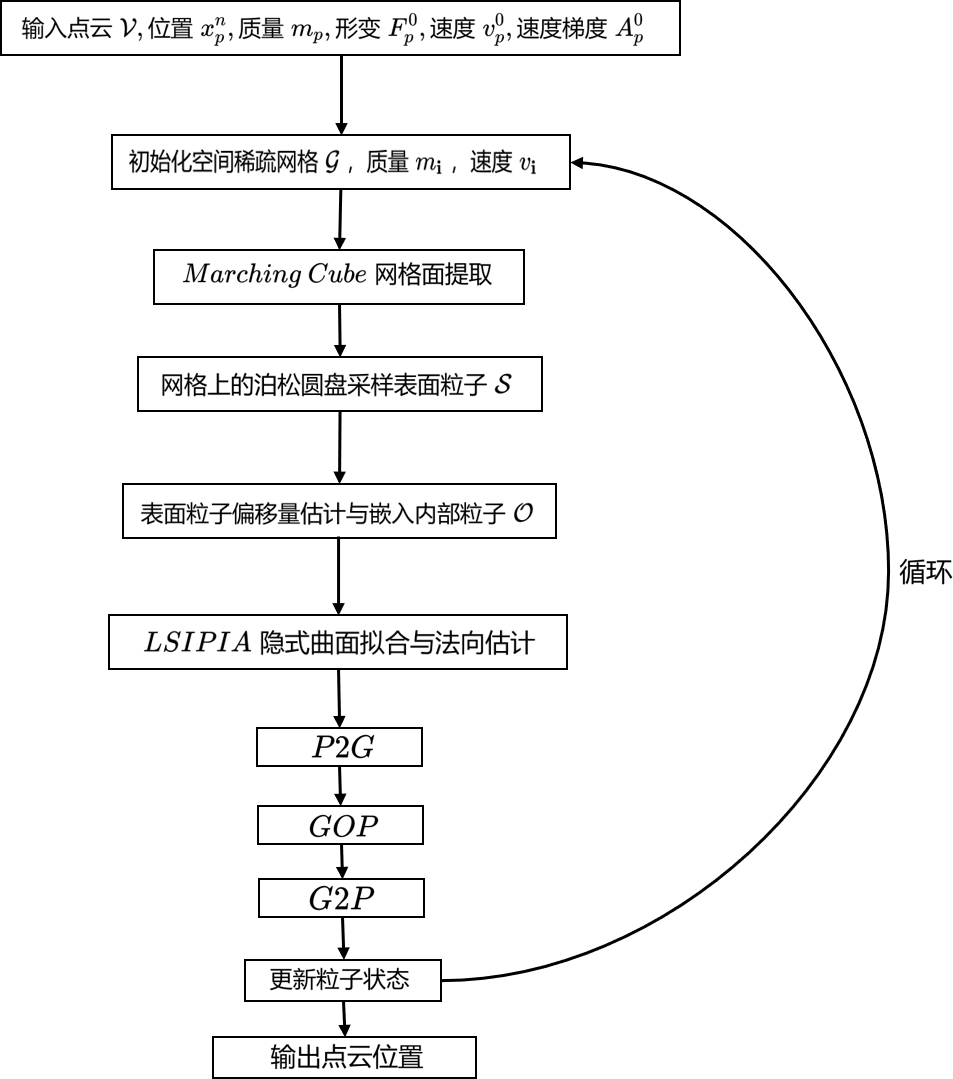
\includegraphics[scale=0.7]{./images/image17.png}
    \caption{计算流水线}
    \label{fig: pipline}
\end{figure}
\section{实验结果}

